\documentclass[12pt]{report}

\usepackage{longtable}
\usepackage{xcolor}
\usepackage{tikz}
\usepackage{stix}
\usepackage[T1]{fontenc}
\usepackage{amssymb,amsmath,mathrsfs,amsthm}
\usepackage{setspace,xurl,tikz-cd,booktabs,placeins}
\usepackage{enumerate}
\usepackage{tocbibind}


\thispagestyle{empty} % remove page number from first page
\definecolor{darkgreen}{RGB}{0,100,0}

\usepackage{natbib}

\widowpenalty10000
\clubpenalty10000

\usepackage[height=8in]{geometry}

\usepackage{hyperref}
\hypersetup{colorlinks=true,
			urlcolor=blue,
			linkcolor=black,
			citecolor=blue,
			bookmarksdepth=paragraph}
			
\usepackage[noabbrev]{cleveref}
\crefname{equation}{}{}

\usepackage[all]{hypcap}  % Make hyperlinks to top of figure, not to caption.
\usepackage{listings}  % Code listings

\newcommand{\bu}{\textbf{u}}
\newcommand{\lap}{\Delta}
\newcommand{\grad}{\nabla}
\newcommand{\ul}{\textbf}
\newcommand{\eps}{\epsilon}

\graphicspath{ {./images/} }
% To prevent "overfull \vbox" error caused by splitting footnotes across pages.
\interfootnotelinepenalty=1000


\hypersetup{
  pdfauthor={Uvic Student},
  pdftitle={Title of the thesis},
  pdfkeywords={thesis, uvic},
}

\renewcommand{\bibname}{References}
\linespread{1.5}
\begin{document}


\pagenumbering{roman}
\setcounter{page}{1} % Reset page counter for Roman numerals


\newpage
{\singlespacing

\begin{center}
{\Large \textbf {Title of the thesis}}
\vspace{2em}

by\\
Uvic Student\\
B.Sc., University of somewhere, 1970

\vspace{2em}

A Thesis Submitted in Partial Fulfillment of the\\
Requirements for the Degree of

\vspace{1em}
MASTER OF SCIENCE
\vspace{1em}

in the Department of Mathematics and Statistics

\vfill

\copyright\; Uvic Student, 2024\\
University of Victoria

\vspace{1em}
All rights reserved. This thesis may not be reproduced in whole or in part, by photocopy or other means, without the permission of the author.
\end{center}
}

\newpage



{\singlespacing
\begin{center}
{\Large \textbf {Title of the thesis}}
\vspace{2em}

\addcontentsline{toc}{section}{Supervisory Committee}



by\\
Uvic Student\\
B.Sc., University of somewhere, 1970
\end{center}

\vfill
\begin{spacing}{0.4}

\noindent \textbf{Supervisory Committee}
\vspace{2em}

\noindent Dr. soandso\\
(Department of Mathematics and Statistics, University of Victoria)
\par\noindent\rule{\textwidth}{0.8pt}
{\small \textbf{Supervisor}}
\vspace{1em}

\noindent Dr. suchandsuch\\
(Department of Mathematics and Statistics, University of Victoria)
\par\noindent\rule{\textwidth}{0.8pt}
{\small \textbf{Committee Member}}
\vspace{1em}

\end{spacing}
\vfill
}

\newpage
\begin{center}
    \Large \textbf{Abstract}
\end{center}
\addcontentsline{toc}{section}{Abstract}
This is a thesis on the topic of blah. Here is a quick summary of what it contains. You will learn many things by reading it.


\newpage
\tableofcontents
\listoftables
\listoffigures



\newpage
\addcontentsline{toc}{section}{Acknowledgments}
\begin{center}
    \Large \textbf{Acknowledgments}
\end{center}
I'd like to thank many people, but I want to keep this short so I'll stick to just a few. First I'd like to thank ...






\newpage
\chapter{Title of the first chapter}

\pagenumbering{arabic}
\setcounter{page}{1} % Reset page counter for Arabic numerals


This is the first chapter, here we will lay out some ideas as well as review some literature. In particular, it is natural to first begin with \citep{the10rules} and \citep{theBook}.


\section{First section of first chapter}
Here is the first labeled section of this chapter. Here is an equation:


\begin{subequations}
\label{the equation}
\begin{align}
x &= y,\\
40 + 2 &= 42
\end{align}
\end{subequations}

as you can see in \label{the equation}, mathematicians like the letters $x$ and $y$.


\section{the second section}

And here in section two of the first chapter, we can see a very nice paragraph.

Very nice. Very nice indeed. Very nice. Very nice indeed. Very nice. Very nice indeed. Very nice. Very nice indeed. Very nice. Very nice indeed. Very nice. Very nice indeed. Very nice. Very nice indeed. Very nice. Very nice indeed. Very nice. Very nice indeed. Very nice. Very nice indeed. Very nice. Very nice indeed. Very nice. Very nice indeed. Very nice. Very nice indeed. Very nice. Very nice indeed. Very nice. Very nice indeed. Very nice. Very nice indeed. Very nice. Very nice indeed. Very nice. Very nice indeed. Very nice. Very nice indeed. Very nice. Very nice indeed. Very nice. Very nice indeed. Very nice. Very nice indeed. Very nice. Very nice indeed. Very nice. Very nice indeed.












\chapter{The second chapter}

And now we cant help but introduce a table. Here you go.


\begin{table}[t]
\centering
\noindent\hrulefill\\
\begin{tabular}{ccccc}
col 1 & col 2 & col 3 & col 4 & col 5 \\
val 1 & val 2 & val 3 & val 4 & val 5 \\
5 & 6 & 7 & 8 & 9 \\
\end{tabular}
\\\noindent\hrulefill\\
\caption[This is a table]{This is a description of the table.}
\label{table1}
\end{table}

As you can see in \label{table1}, tables are very nice to look at.


\chapter{Chapter 3}
In this 3rd chapter, we discuss some ideas before proceeding to the first section.


\section{First section of chapter 3}
In this first section of chapter 3, let us begin with a very nice paragraph.


Very nice. Very nice indeed. Very nice. Very nice indeed. Very nice. Very nice indeed. Very nice. Very nice indeed. Very nice. Very nice indeed. Very nice. Very nice indeed. Very nice. Very nice indeed. Very nice. Very nice indeed. Very nice. Very nice indeed. Very nice. Very nice indeed. Very nice. Very nice indeed. Very nice. Very nice indeed. Very nice. Very nice indeed. Very nice. Very nice indeed. Very nice. Very nice indeed. Very nice. Very nice indeed. Very nice. Very nice indeed. Very nice. Very nice indeed. Very nice. Very nice indeed. Very nice. Very nice indeed. Very nice. Very nice indeed. Very nice. Very nice indeed. Very nice. Very nice indeed. Very nice. Very nice indeed.

And then follow up with \label{cats}, a picture of some cats.

\begin{figure}[htbp]
\begin{center}
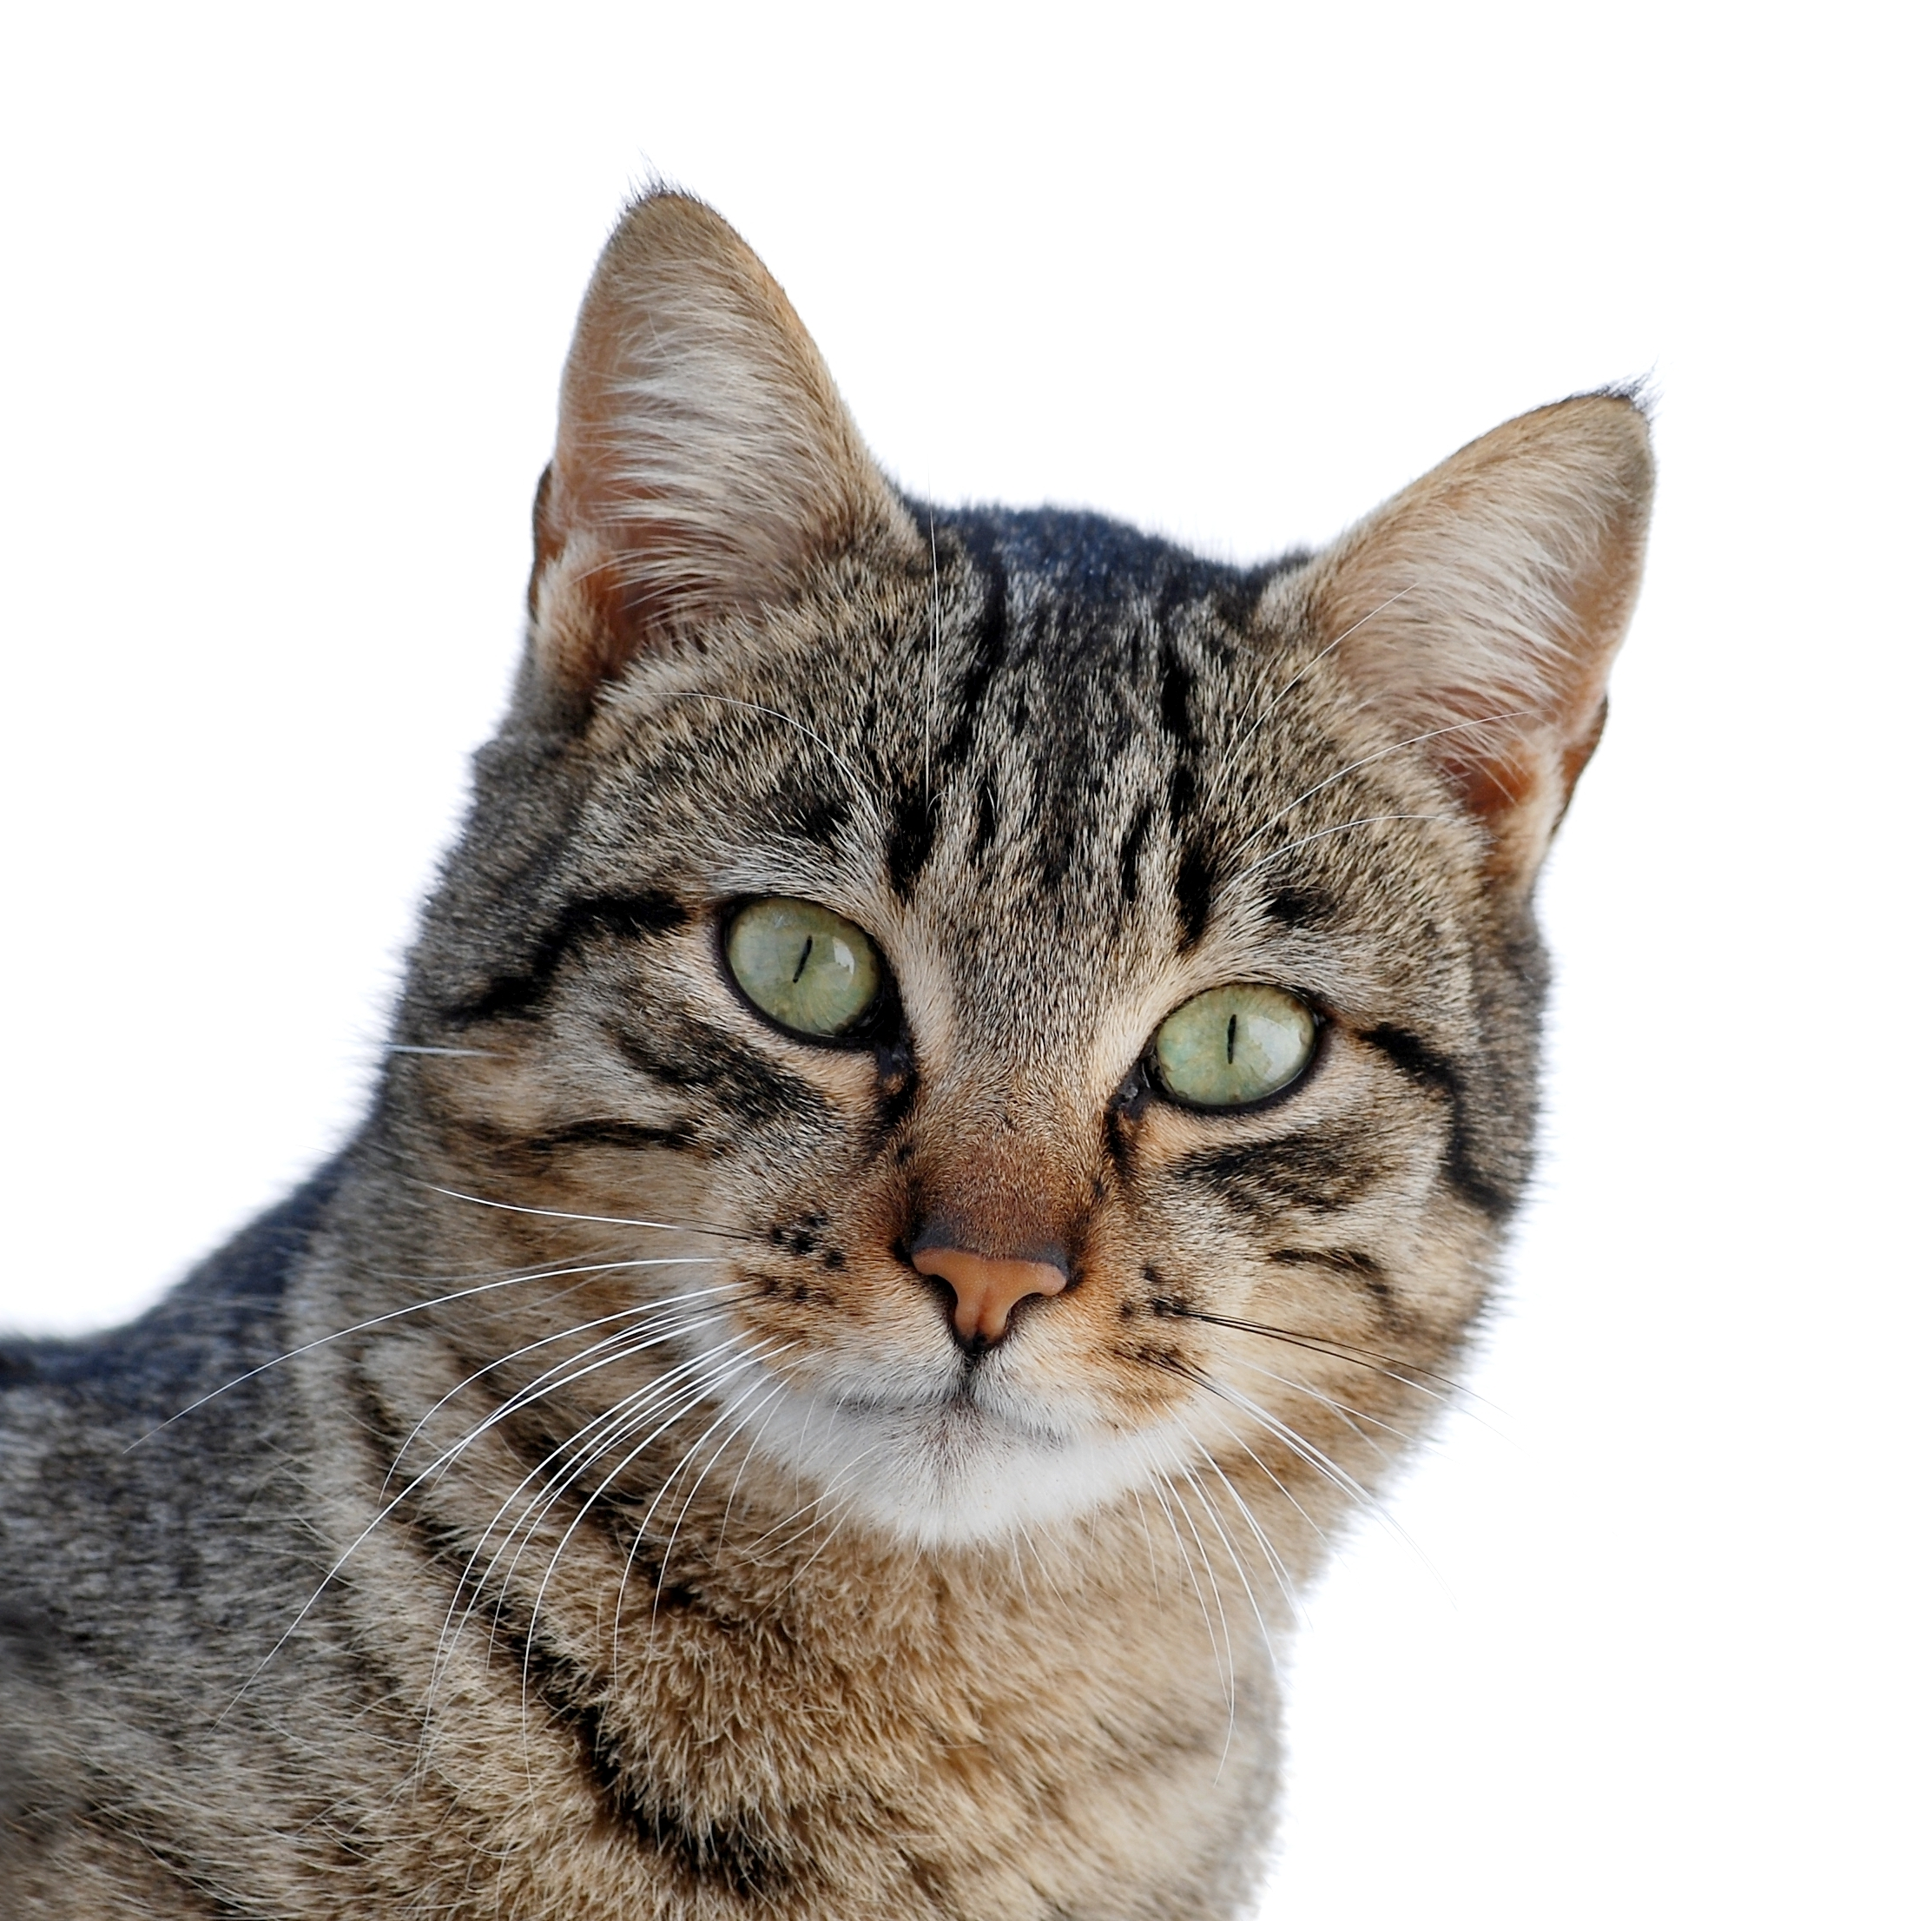
\includegraphics[height=.08\textheight]{cat.jpg}
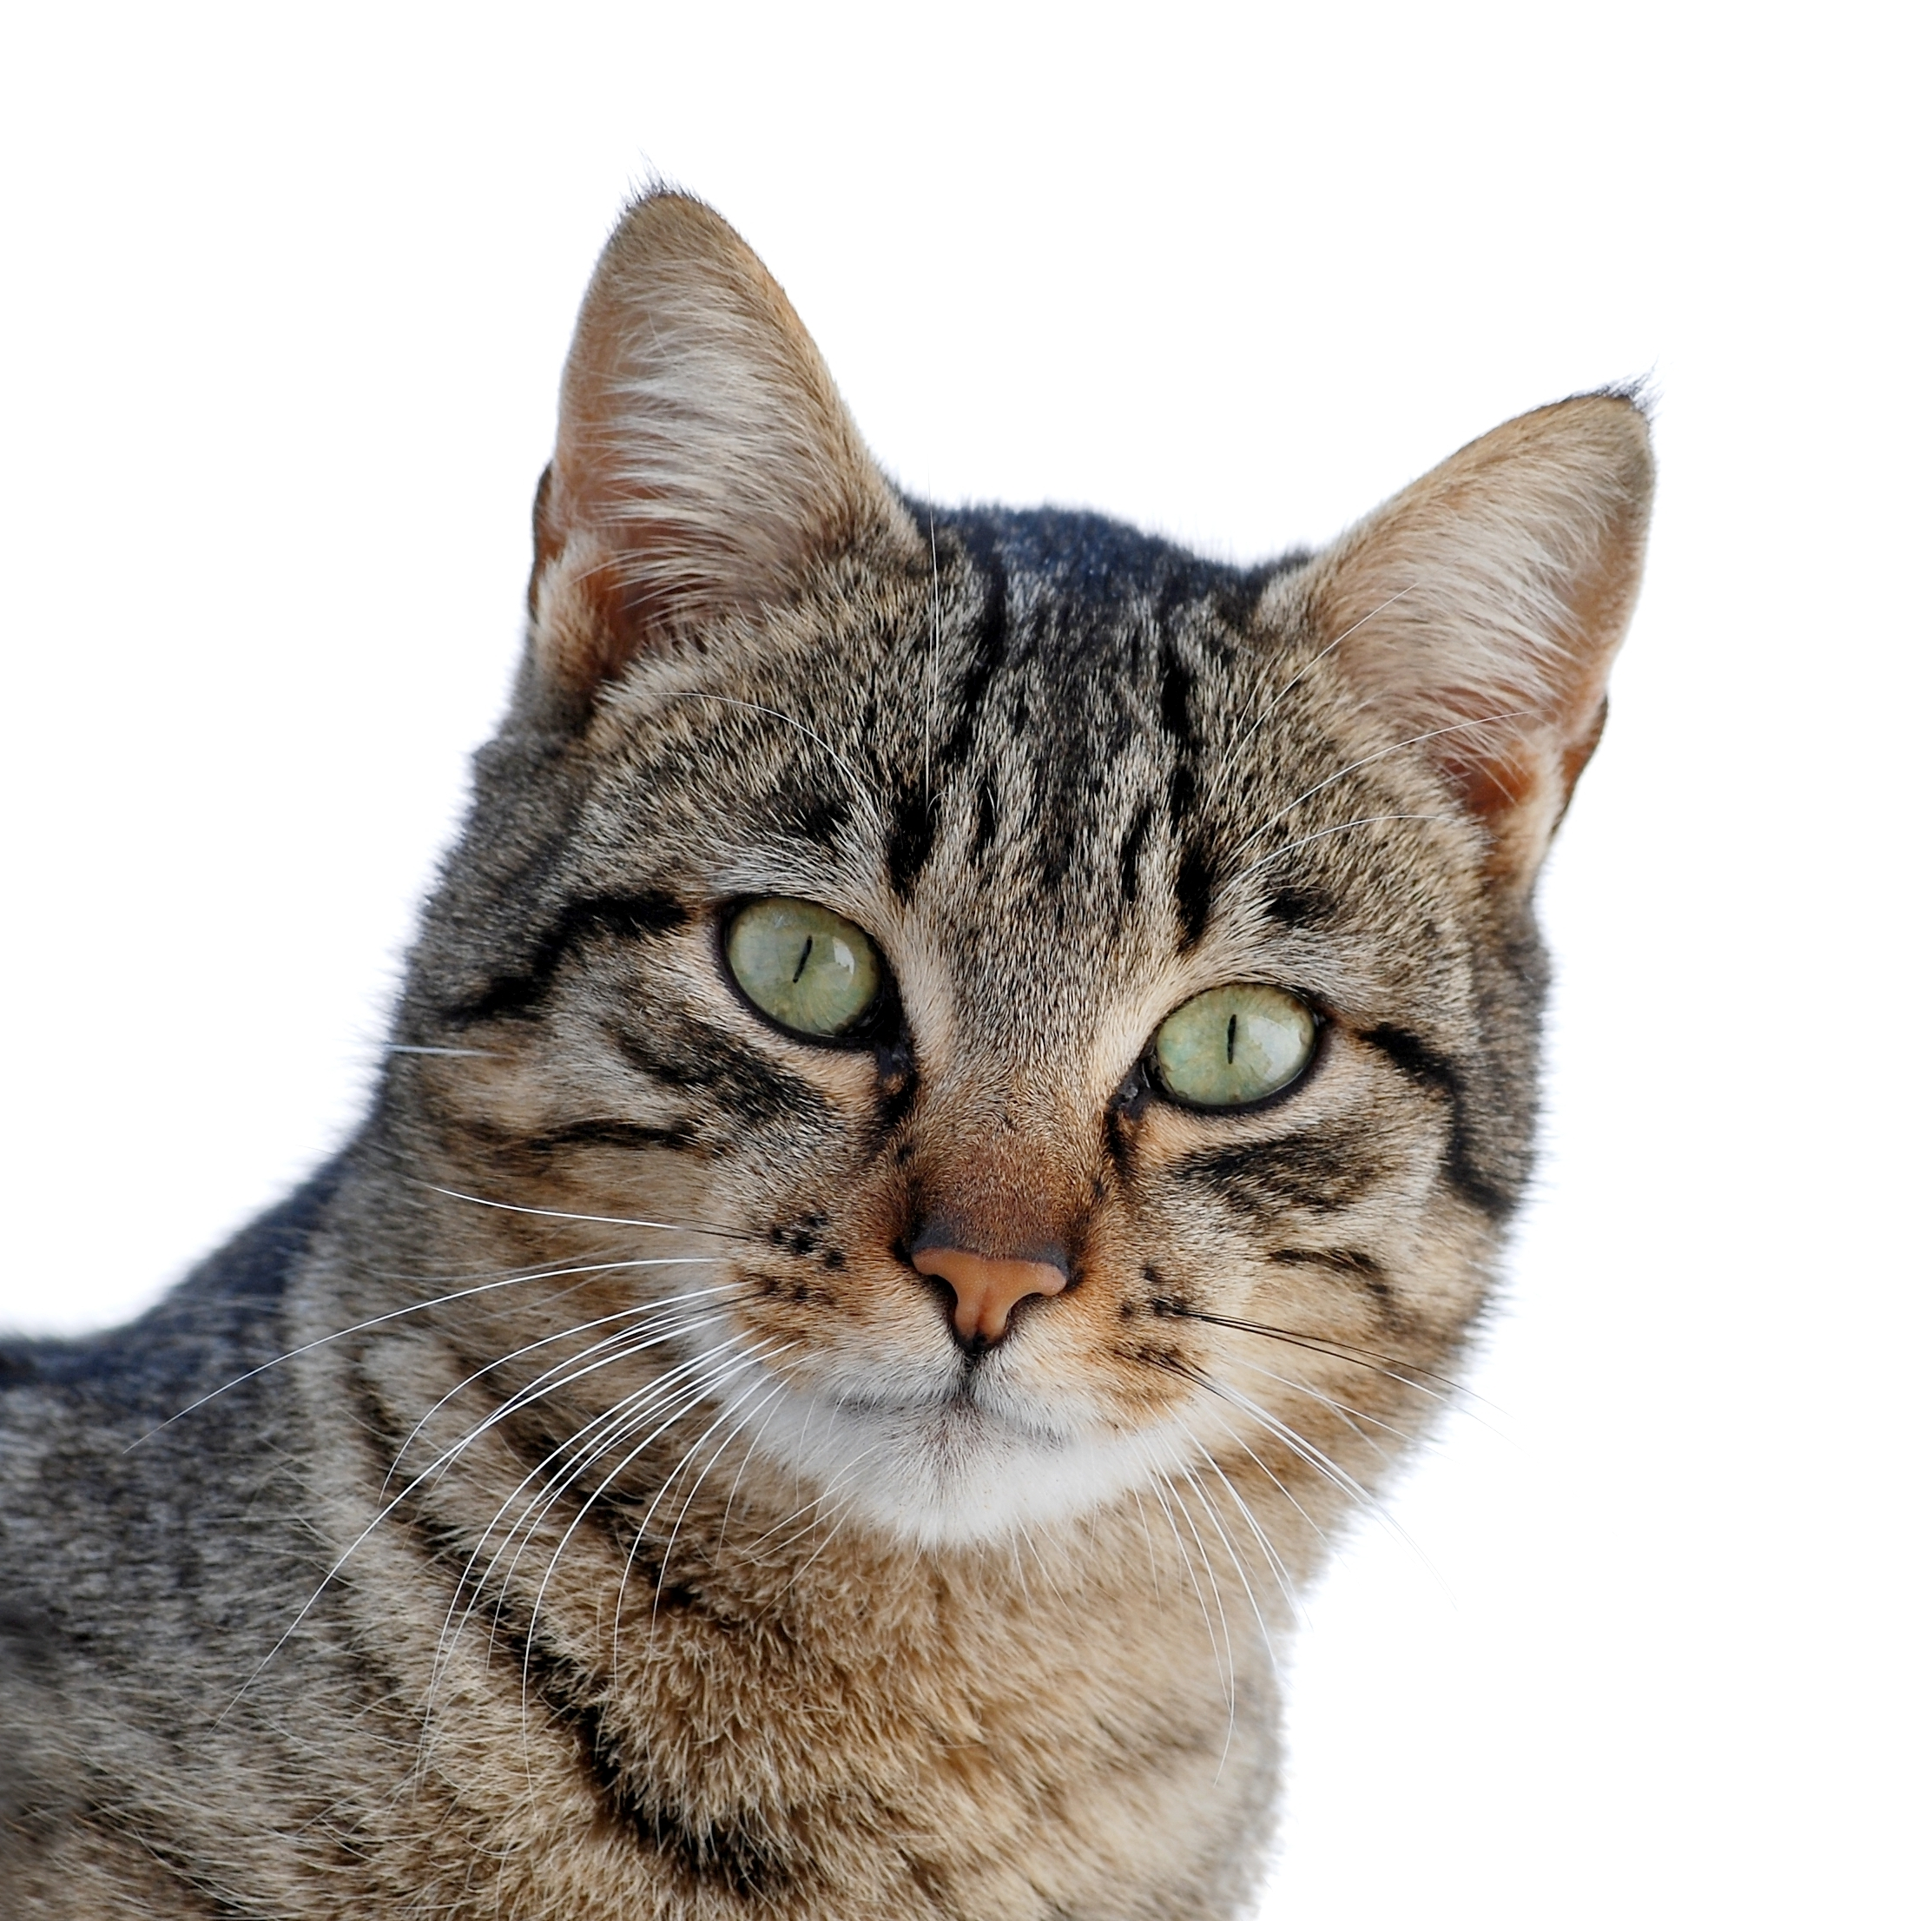
\includegraphics[height=.08\textheight]{cat.jpg}
\caption[some cats]{Despite their similarities, the first and second cat are actually slightly different. Can you spot how?}
\end{center}
\label{cats}
\end{figure}


\chapter{Discussion and future work}
This is a concluding section, we discuss our findings and then proceed to say what we would like to do in the future.


\bibliographystyle{plainnat}
\bibliography{references}

\appendix
\chapter{appendix}
\label{sec:appendix_code}

This is an appendix containing additional content which doesn't fit nicely in the rest of the thesis. If you have some code, maybe consider putting it here?


\end{document}







